\subsection{Gradient Variance of the Walk Ansatz}
\label{sec:gradvar}

Every variational result in this chapter was obtained with a derivative-free
optimiser under a fixed budget, so a model that fails to improve may be
failing because its landscape is flat or because the optimiser never reached
the region where it is not. The quantity that separates the two is the
variance of the gradient at random parameters, whose exponential decay in the
number of qubits defines a barren plateau~\cite{McClean_2018, Larocca_2025}.
It is measured here in two ways. Both draw every parameter uniformly from
$[0, 2\pi)$, differentiate with respect to eight randomly chosen parameters
per draw over 200 draws, and report the variance with a bootstrap
$95$ per cent interval. Gradients are central finite differences on the exact
state vector, checked against the exact parameter-shift rule on the
hardware-efficient ansatz to within $3e-10$.

\paragraph*{Depth, on the classifier's own register.}
The first measurement uses the classifier of Section~\ref{sec:qnnmethod}
unchanged: the same training loss, the same five-qubit states produced by two
steps of the real walk feature map on the $140$ training images, and the same
observable $Z^{\otimes 5}$, so that only the ansatz varies. Three ansätze
are compared at depths $1$ to $32$: the walk ansatz with a real coin and with
a complex coin, and a hardware-efficient ansatz of $R_Y$ rotations, a CNOT
ladder and $R_X$ rotations on the same five qubits.
Figure~\ref{fig:gradvar}(a) gives the result. None of the three decays with
depth. The real-coin walk ansatz holds between $7.6 \times 10^{-3}$ and
$8.5 \times 10^{-3}$ across all depths, above the hardware-efficient ansatz's
$3.7 \times 10^{-3}$ to $5.7 \times 10^{-3}$; the complex-coin ansatz sits
2.2 to 2.6 times lower than the real one at every
depth. At the depths the classifiers actually use, two and four steps, the
walk ansatz therefore has gradients at least as large as a standard ansatz on
the same register, and the results of Section~\ref{sec:qnnresults} are not
the product of a vanishing gradient. The complex arm here is the trained-phase
ansatz after the real feature map, the configuration in which the complex coin
fits worse at equal parameter count; its smaller per-parameter gradient is
consistent with that, though it does not by itself explain it, and says
nothing about the complex feature map, with which the sign of the effect
reverses.

\paragraph*{Width, on graphs of increasing size.}
Five qubits cannot exhibit a barren plateau, since the phenomenon is decay in
the number of qubits. For a walk that number is set by the graph, $\log_2 N +
\log_2 d$, so the second measurement varies the graph: grids of $8$ to
$1024$ vertices, giving registers of $5$ to $12$ qubits, each walked for
$R + C$ steps from the uniform arc state with no data, so that the ansatz is
isolated as in~\cite{McClean_2018}. Two walk ansätze are compared, the
per-vertex coin of axis~1, with an independent angle at every vertex and
step, and the per-step coin of axis~2, with one angle per step shared by all
vertices, against the hardware-efficient ansatz of the same width and depth.
Because a cost measured on every qubit is known to flatten even shallow
circuits~\cite{Larocca_2025}, both the classifier's global observable
$Z^{\otimes n}$ and a local one, $Z$ on a single qubit, are reported.
Figure~\ref{fig:gradvar}(b,c) and Table~\ref{tab:gradvar} give the result.

The two walk ansätze behave in opposite ways. Under the local cost the
per-vertex coin loses a factor of about $5.1$ in variance per added
qubit, against about $2.0$ for the hardware-efficient ansatz; since the
register grows as $\log_2 N$, this is a variance falling as
$N^{-2.0}$ to
$N^{-2.3}$ (global and local cost) in the size
of the graph --- polynomial in $N$, but exponential in the
qubit count, and faster than the generic ansatz. The mechanism is locality:
each angle rotates the coin at one vertex at one step, and so acts on a share
of the amplitude of order $1/N$. The per-step coin does the reverse. Its
angle acts at every vertex at once, and under the local cost its variance
falls by a factor of only about 7 between $5$ and
$12$ qubits --- a fitted slope of $-0.31$ in
$\log_2 \mathrm{Var}$ per qubit, noisy at the largest sizes --- against
about 120 for the hardware-efficient ansatz and
about 110\,000 for the per-vertex coin. At $12$
qubits it stands at $3.6 \times 10^{-2}$, against $1.2 \times 10^{-4}$ and $2.6 \times 10^{-7}$
respectively. Under the global cost every ansatz
decays, the per-step coin included, which is the global-cost mechanism rather
than a property of the walk.

Three consequences follow. The first is that the per-vertex parameterisation
of axis~1 --- the one the classifier's walk ansatz uses --- fails at scale
for a second, independent reason: its gate count grows as $N^{3.1}$
(Section~\ref{sec:depth}), and its gradient variance shrinks as about
$N^{-2}$. The second
is that the per-step coin of axis~2, which the resource analysis already
favoured because it costs nothing in width or depth, is also the one that
keeps a usable gradient as the graph grows, provided the read-out is local.
The third is that the classifier's global read-out $Z^{\otimes n}$ would have
to be replaced by a local one before the construction could be trained at
any size larger than the one used here. The measurement has limits that
should be stated with it: it is taken at random parameters, not along the
path an optimiser follows; it uses grid graphs only, up to $12$ qubits; it
uses the real rotation coin, not the Grover-exponential coin of the graph
walk network; and it does not replace a training run with gradients, so the
negative results of this chapter about trainable coins remain conditional on
the derivative-free budget under which they were obtained.

\begin{figure}[htbp]
  \centering
  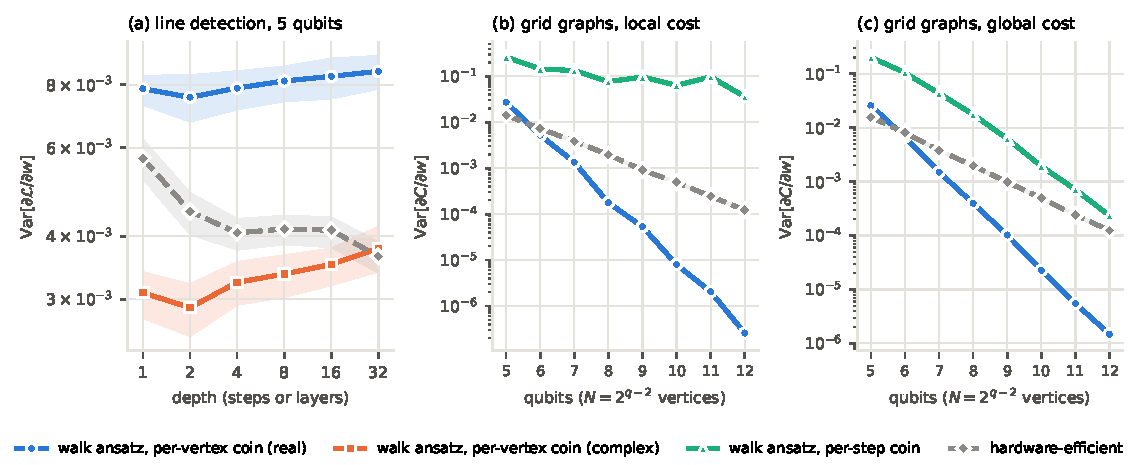
\includegraphics[width=\textwidth]{fig_gradient_variance.pdf}
  \caption[Gradient variance of the walk ansatz]{Variance of the gradient
  with respect to one ansatz parameter at uniformly random parameters, with
  bootstrap $95$ per cent bands. (a)~Against depth, on the five-qubit
  line-detection register with the classifier's loss and observable; only the
  ansatz differs. (b,c)~Against register width on grid graphs of $8$ to
  $1024$ vertices, at depth $R + C$ and without data, for a local and a
  global cost. The per-vertex coin gives each angle one vertex; the per-step
  coin shares one angle across all vertices.}
  \label{fig:gradvar}
\end{figure}

\begin{table}[htbp]
\centering\small
\caption[Gradient variance of the walk ansatz against register width]{Variance of the gradient of the cost with respect to one ansatz parameter, over 200 uniformly random parameter draws, on grid graphs of increasing size at depth $T = R + C$. Local cost: $Z$ on the most significant qubit; global cost: $Z$ on every qubit, the classifier's observable. The last row is the least-squares slope of $\log_2 \mathrm{Var}$ per added qubit.}
\label{tab:gradvar}
\setlength{\tabcolsep}{4pt}
\begin{tabular}{rrrrrrrr}
\hline
 & & \multicolumn{3}{c}{local cost} & \multicolumn{3}{c}{global cost} \\
Grid & Qubits & per-vertex & per-step & HEA & per-vertex & per-step & HEA \\
\hline
2$\times$4 & 5 & $2.7\times10^{-2}$ & $2.6\times10^{-1}$ & $1.4\times10^{-2}$ & $2.6\times10^{-2}$ & $2.0\times10^{-1}$ & $1.6\times10^{-2}$ \\
4$\times$4 & 6 & $5.2\times10^{-3}$ & $1.4\times10^{-1}$ & $7.3\times10^{-3}$ & $6.7\times10^{-3}$ & $1.0\times10^{-1}$ & $8.1\times10^{-3}$ \\
4$\times$8 & 7 & $1.4\times10^{-3}$ & $1.3\times10^{-1}$ & $3.9\times10^{-3}$ & $1.5\times10^{-3}$ & $4.3\times10^{-2}$ & $3.8\times10^{-3}$ \\
8$\times$8 & 8 & $1.8\times10^{-4}$ & $7.7\times10^{-2}$ & $2.0\times10^{-3}$ & $3.9\times10^{-4}$ & $1.8\times10^{-2}$ & $2.0\times10^{-3}$ \\
8$\times$16 & 9 & $5.3\times10^{-5}$ & $9.7\times10^{-2}$ & $9.1\times10^{-4}$ & $1.0\times10^{-4}$ & $6.2\times10^{-3}$ & $9.8\times10^{-4}$ \\
16$\times$16 & 10 & $8.0\times10^{-6}$ & $6.4\times10^{-2}$ & $5.0\times10^{-4}$ & $2.3\times10^{-5}$ & $1.9\times10^{-3}$ & $4.9\times10^{-4}$ \\
16$\times$32 & 11 & $2.1\times10^{-6}$ & $9.8\times10^{-2}$ & $2.4\times10^{-4}$ & $5.5\times10^{-6}$ & $7.1\times10^{-4}$ & $2.4\times10^{-4}$ \\
32$\times$32 & 12 & $2.6\times10^{-7}$ & $3.6\times10^{-2}$ & $1.2\times10^{-4}$ & $1.5\times10^{-6}$ & $2.3\times10^{-4}$ & $1.2\times10^{-4}$ \\
\hline
\multicolumn{2}{l}{slope} & $-2.35$ & $-0.31$ & $-0.98$ & $-2.02$ & $-1.42$ & $-1.00$ \\
\hline
\end{tabular}
\end{table}

